\documentclass{article}
\usepackage[a4paper]{geometry}
\usepackage[english]{babel}
\usepackage[utf8]{inputenc}
\usepackage{url}
\usepackage{hyperref}
\usepackage{graphicx}
\usepackage{amsmath}
\usepackage{amsfonts}
\usepackage{amssymb}
\usepackage{amsthm}
\usepackage{float}

\newcommand{\Sum}[3]{\ensuremath{\displaystyle\sum\limits_{#1}^{#2} #3}}
\newcommand{\scaleFreeFunction}{\ensuremath{p_k = C \cdot k^{-\gamma}}}

\newcommand{\netDescription}[1]{degree distributions in log-log scale of the \textit{net#1} graph. The black points are the data extracted from the graph. The gray dashed line is the curve fit of a power law function \scaleFreeFunction.}

\title{Activity 5}
\author{Lucas Guesser Targino da Silva - RA: 203534}

\begin{document}

\maketitle

\section{Problem Description}

Two undirected networks are given in the \verb|data/| directory of the project. For them:

\begin{enumerate}
    \item Plot their degree distributions in log-log scale
    \item Answer: which of the two is more likely to be a scale-free network?
\end{enumerate}

\section{Result}

As stated in \href{http://networksciencebook.com/chapter/4}{Barabasi's book, Chapter 4 on Scale-Free Property}, the degree distribution of Scale-Free Networks follow the Power Law given by \scaleFreeFunction.

Comparing the Figures \ref{figure:net1} and \ref{figure:net2}, one notices that the network of the \textit{net1} data set fits better the give Scale-Free Network model. Therefore, \textit{net1} is more likely to be a Scale-Free Network than \textit{net2}.

\begin{figure}[!ht]
    \centering
    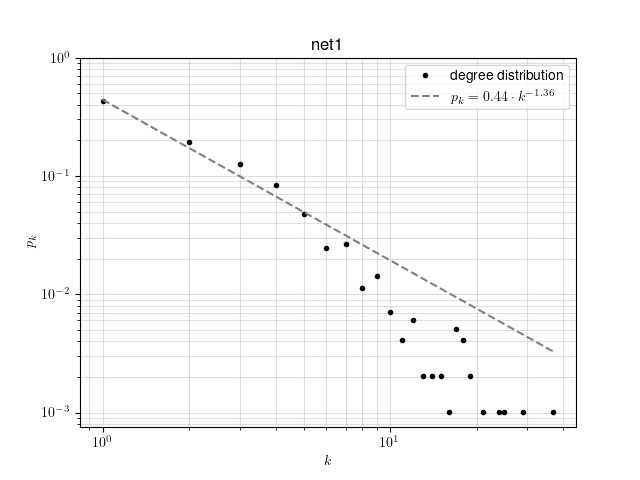
\includegraphics[width=\textwidth]{../result/net1.png}
    \caption{\netDescription{1}}
    \label{figure:net1}
\end{figure}

\begin{figure}[!ht]
    \centering
    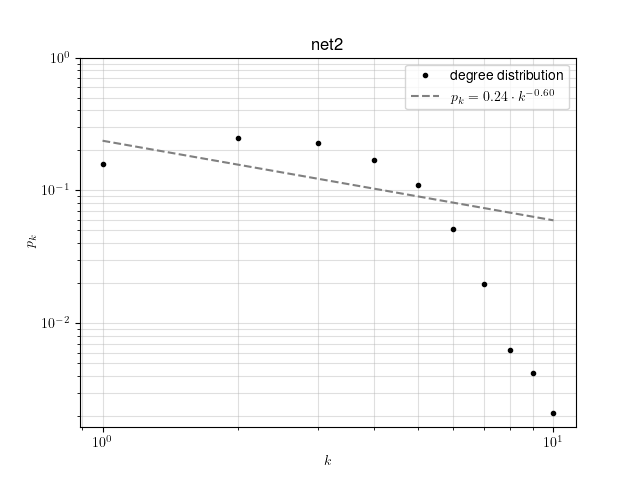
\includegraphics[width=\textwidth]{../result/net2.png}
    \caption{\netDescription{2}}
    \label{figure:net2}
\end{figure}

\end{document}
